%!TEX root = ../master.tex
\section{Semantic technologies}
The \emph{Semantic Web} is a vision made by Tim Berners-Lee, an extension of the World Wide Web where information has a formal description and well-defined meaning, making the data more machine-readable—enabling better cooperation between computer and human \autocite{Berner-Lee_The_samantic_web}. The different specification and tools we can utilise for structuring the data in the Semantic Web are called Semantic Technologies. OWL, RDF, RDFS are some well-known Semantic Technologies. Furthermore, the Semantic web structures its data through linked data. Mauro and Tiziana summarised linked data as a means to connect, expose and share web data utilising URIs required for the construction of the Semantic Web\autocite{Mauro_Tiziana_linked_data}. We further elaborate on URIs in \autoref{RDF}. The connections connect different URIs, where the connection, which also is a URI, provides information on the relationship the first identifiers have to the second one. The result will then resemble a directed graph. In addition, the connected data requires some formal semantic to work provided by the Semantic technologies, structuring the linked data by providing a formal description of terms, relationships, and concept in the knowledge domain. In semantic web and computer science in general, we would call this an \emph{ontology}. By definition, an \emph{ontology} is the knowledge we have about a given domain that is machine-processable and with a formally defined meaning \autocite[2]{FOSWT}.

\begin{figure}
    \centering
    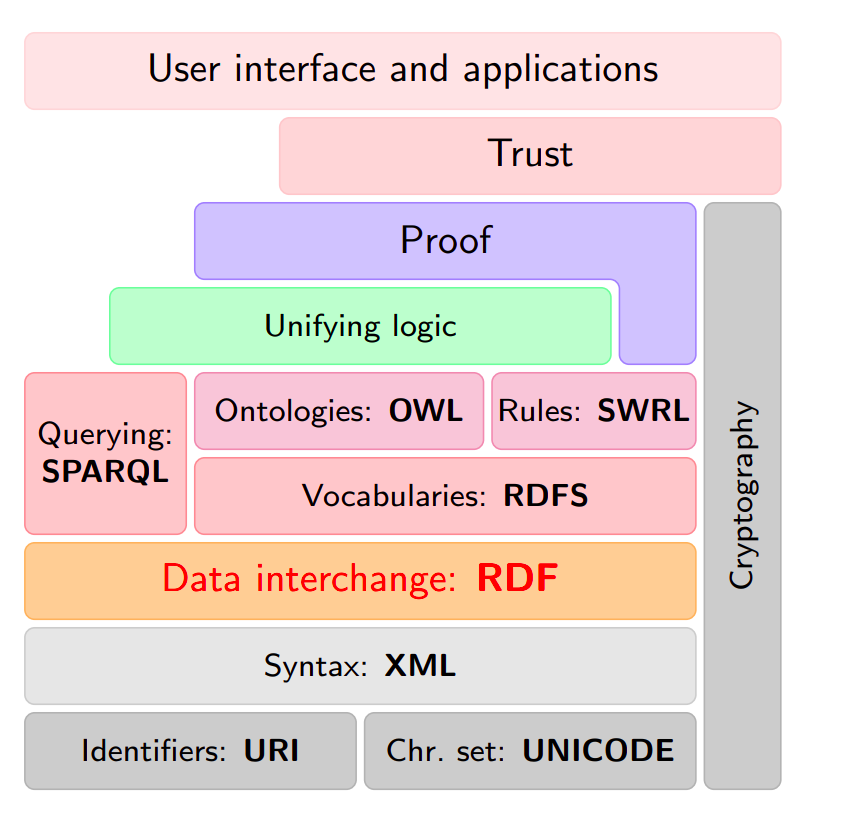
\includegraphics[scale=0.2]{SWStack.png}
    \caption{The semantic web stack src: IN3060 foiler uke 2}
    \label{fig:SW stack}
\end{figure}


\subsection{RDF}
\label{RDF}
RDF stands for \emph{Resource Description Framework} and is a framework for formally describing structure\lhk{typo?} data \autocite[19]{FOSWT}. Furthermore, RDF is the general method used in the semantic web to represent information in a web resource, which describes a collection of triples. As the name triple insinuates, a triple contains three elements, or more formally, three resources. These three resources have unique names and meaning depending on their placement in the triple. Firstly the subject, secondly the predicate and lastly, the object \autocite{W3C_RDF}. The predicate describes a relationship that the subject has to the object. Usually, one can define a collection of triples as a graph where the subjects and objects are nodes, and the predicates are a directed edge from a subject to an object \autocite{W3C_RDF}. However, RDF can represent a structure that we ordinarily would not describe as a graph because there are no restrictions in RDF for a resource being only a subject/object or a predicate. In terms of results, it is possible to have an element in the graph representing a node and an edge. An example of a triple is Sebastian hasFather Thommas, where Sebastian is the object, hasFather is the predicate, and Thommas is the object. RDF have numerous serialization formats; we will use Turtle\lhk{cite Turtle-spec?} for the examples.  

\para
To distinguish between the different resources in an RDF graph, we need to identify the different resources uniquely. Therefore, RDF uses \emph{Uniform Resource Locator} (URI)\lhk{URI is short for Uniform Resource \emph{Identifier}, not \emph{Locator} (that is URL)}, where every URI represent a unique resource \autocite[21-22]{FOSWT}. Every URL is a URI ($URL\subseteq URI$). However, not all URIs are URL ($URL\nsubseteq URI$).  Previously, we had an example triple Sebastian hasFather Thommas. This example needs to use URI since we need to distinguish between the different resources, resulting in the triple $<http://example.org/person/Sebastian> <http://example.org/relation/hasFather> <http://example.org/person/Thommas> .$\lhk{Rather use monospace/verbatim font here, and perhaps put on a new line/new environment} . However, it may become time-consuming to write the whole URI for Sebastian every time we want to refer to the Sebastian resource; therefore, we have something called prefix in Turtle. We need to set the prefixes at the start of the Turtle document. Appending $@PREFIX\; ex-p:\; <http://example.org/person/>.$ in the start of the document containing the example triple would result in the possibility to shorten <http://example.org/person/Sebastian> down to ex-p:Sebastian . Adding the prefix $@PREFIX\; ex-r:\; <http://example.org/relation/>.$ results in the opportunity to shorten the full triple down to $ex-p:Sebastian\; ex-r:hasFather\; ex-p:Thommas\; .$. The examples in the following sections utilies the following prefixes.

\begin{lstlisting}[frame=single, language=turtle]
@prefix  ex-p:  <http://example.org/person/> . 
@prefix ex-r:  <http://example.org/relation/> . 
@prefix ex-t:  <http://example.org/template/> . 
@prefix xsd: <http://www.w3.org/2001/XMLSchema/#>  . 
@prefix rdf: <http://www.w3.org/1999/02/22-rdf-syntax-ns#> .
@prefix ottr: <http://ns.ottr.xyz/0.4/> .
@prefix o-rdf: <http://tpl.ottr.xyz/rdf/0.1/> .
\end{lstlisting}

\para
In the previous examples, we have started to make an ontology for families. Sometimes we know something about something without knowing what that thing is. For example, we may know that Sebastian has a father without knowing how the father is. RDF uses \emph{blank nodes} to express that we know something about a resource without knowing the URI of the resource. In the case when we know that Sebastian has a father without knowing who the father is the father is a blank node. Note that a blank node can only  occur in the subject or object position, not in the predicate position. To model that Sebastian has a father we can write either $ex-p:Sebastian\; ex-r:hasFather\; \_:b .$ or $ex-p:Sebastian\; ex-r:hasFather\; [\; ]$ , beacause the syntax for writing a blank node in Turtle is either $\_:<some variable name>$ or $[\; ]$. Since an blank node also can be a subject, we can express things about the blank node. Therefore, if we want to model that Sebastian has a father who also has a father who is http://example.org/person/Roger we can write $ex-p:Sebastian\; ex-r:hasFather\; [\; ex-r:hasFather\; ex-p:Roger] .$ or $ex-p:Sebastian\; ex-r:hasFather\; \_:father . \\ \_:father \; ex-r:hasFather\; ex-p:Roger .$

\para
RDF also uses \emph{literals}, such as strings and integers \autocite{W3C_RDF}. Literals can only be in the object position of the triple. If we want to express that Sebastian has age 22 we can write $ex-p:Sebastian\; ex-r:hasAge\; " 22 " <opp greie> <opp greie> xsd:int.$\lhk{If you use verbatim-font here, you can of course just write the carot/"oppgreie" directly, however, if you want it in math-mode, you can write $\hat{\ }\hat{\ }$} . In addition, we can add that Sebastian has the name Sebastian in Norweigan and Bastian in English by using \emph{language tags}. Expressing the different names in RDF, results in the triples $ex-p:Sebastian\; ex-r:hasName\; Sebastian@no.$ and $ex-p:Sebastian\; ex-r:hasName\; Bastian@en.$. The graph containing all the triples we mention in this section, by now, looks like this:

\begin{lstlisting}[frame=single, language=turtle]
ex-p:Sebastian ex-r:hasFather ex-p:Thommas .
ex-p:Sebastian ex-r:hasFather [ ex-r:hasFather ex-p:Roger] . 
ex-p:Sebastian ex-r:hasAge  "22"^^xsd:int . 
ex-p:Sebastian ex-r:hasName  "Sebastian"@no . 
ex-p:Sebastian ex-r:hasName  "Bastian"@en .
\end{lstlisting}

\para
In addition, to the already mentioned abbreviations, Turtle has some more abbreviations to make the Turtle file more compact. For instance, if we have the same predicate and subject several times, with different objects, we can write the predicate and subject one time and separate the objects with a comma (,). Furthermore, Turtle also allows us to abbreviate when we use the same subject several times by writing semicolon (;) at the end of the line instead of dot(.). The aforementioned abbreviations produce the following turtle file:

\begin{lstlisting}[frame=single, language=turtle]
ex-p:Sebastian ex-r:hasFather ex-p:Thommas, [ ex-r:hasFather ex-p:Roger] ; 
                ex-r:hasAge  "22"^^xsd:int ; 
                ex-r:hasName  "Sebastian"@no, "Bastian"@en .
\end{lstlisting}
\autoref{fig:exampelGraph} is a visualization of the graph we have now made.

\begin{figure}
    \centering
    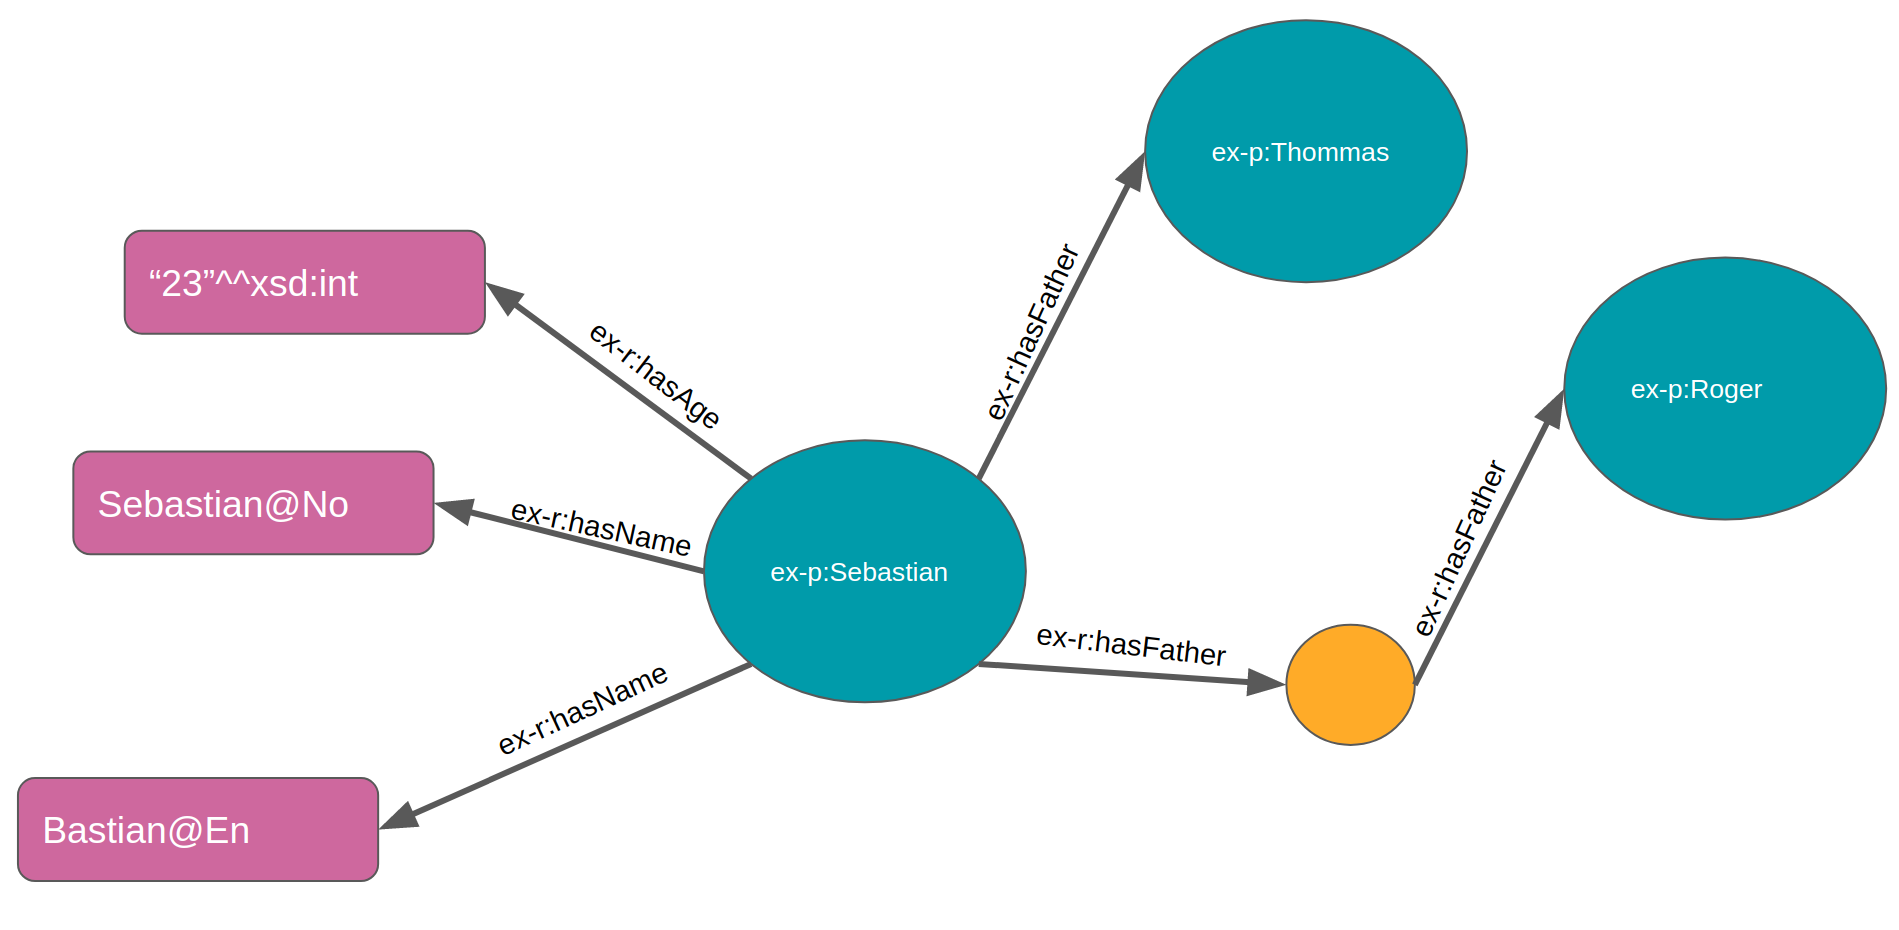
\includegraphics[scale=0.2]{exampleGraph.png}
    \caption{The visual graph over the graph made in section 2.1}
    \label{fig:exampelGraph}
\end{figure}

\subsubsection{Lists in RDF}
In RDF, we have two main ways to represent lists, \emph{containers} and \emph{collections} \autocite[58-63]{FOSWT}. These two are approaches to link data together using blank nodes.

\para
Firstly, a container has three different types, namely rdf:Seq (represents an order list), rdf:Bag (representing an unordered set) and rdf:Alt (representing a set of alternatives). A blank node with a rdf:type rdf:Seq, rdf:Bag or rdf:Alt builds up a container. As long as the container is one of the three types, it does not change its structure, only how the different applications display the container. To add nodes to the container, we need to add a predicate, $rdf\_1$ to $rdf\_n$, from the blank node to the element. Where the first element has the predicate $rdf\_1$, and the n-th element has predicate $rdf\_n$. The following RDF graph shows Sebastians ancestors in an unordered set:\footnote{Note that we have used the abbreviation a for rdf:type}:
\begin{lstlisting}[frame=single, language=turtle]
ex-p:Sebastian ex-r:hasFather ex-p:Thommas, [ ex-r:hasFather ex-p:Roger] ; 
                ex-r:hasAge  "22"^^xsd:int ; 
                ex-r:hasName  "Sebastian"@no, "Bastian"@en ;
                ex-r:ancestor [a rdf:Bag; 
                                rdf:_1 ex-p:Thommas; 
                                rdf:_2 ex-p:Roger].
\end{lstlisting}
Secondly, we can make lists by using collections. The main difference between a container and a collection is that a collection is closed, meaning it is impossible to add new elements after making a list. On the contrary, it is possible to add new elements to a container, as long as we reference the blank node (e.g. \_:list). The reason for collections being closed is that they are built up like a linked list where we connect blank nodes, which links to an element. Collections have two predicates to link the blank nodes and elements together. 

\begin{itemize}
    \item rdf:first: is the predicate linking us to an element
    \item rdf:rest: linking us to the rest of the list
    \item rdf:nil: end of the list
\end{itemize}
\autoref{fig:containerAndCollection} visualises the differences between containers and collections. In Turtle, we can use () as an abbreviation for writing collections where we put the collection elements inside the (). In the general case, a collection will look like this $(member_1 \;member_2 .... member_n)$ An RDF graph containing Sebastian's ancestors using a collection ends up looking like this:

\begin{lstlisting}[frame=single, language=turtle]
ex-p:Sebastian ex-r:hasFather ex-p:Thommas, [ ex-r:hasFather ex-p:Roger] ; 
                ex-r:hasAge  "22"^^xsd:int ; 
                ex-r:hasName  "Sebastian"@no, "Bastian"@en ;
                ex-r:ancestor (ex-p:Thommas ex-p:Roger).
\end{lstlisting}

\begin{figure}
    \centering
    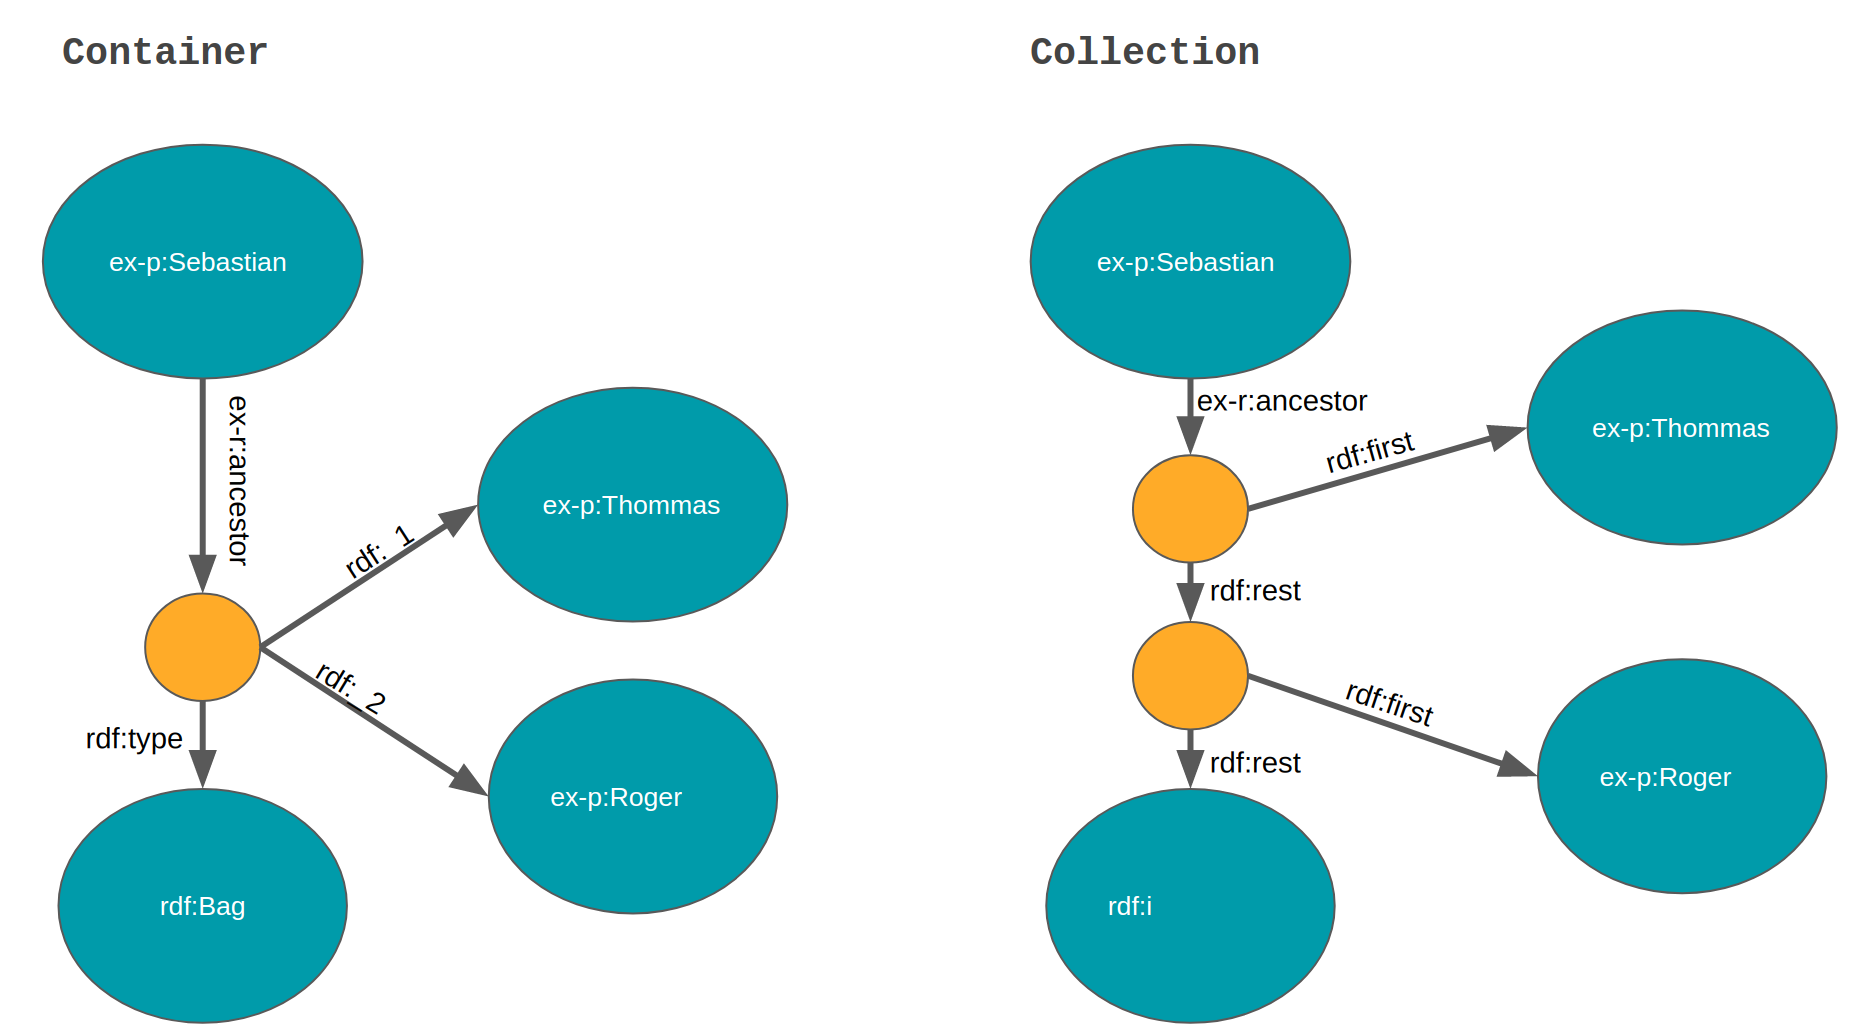
\includegraphics[scale=0.2]{containerAndCollection.png}
    \caption{Shows the difference between a container and a collections in structur}
    \label{fig:containerAndCollection}
\end{figure}

\subsection{OTTR}
\emph{Reasonable Ontology Templates} OTTR is a language representing ontology modelling patterns as parameterised ontologies and can make user-defined abstractions to recurring modelling patterns \autocite[477]{SLKF_OTTR_2018}. OTTR has two central constructors, \emph{templates} and \emph{instances} \autocite[3]{SLKK_OTTR_2021}. The OTTR  templates consist of a head and a body, where the head specifies a templates' name and parameters, whereas the body contains the parameterised ontology pattern \autocite[479]{SLKF_OTTR_2018}. In addition, OTTR allows us to determine the types, which \autoref{ottr types} discusses, and the cardinality of the parameters. There are two types of cardinalities \emph{mandatory} or \emph{optional}. Optional is denoted with a ? while mandatory is the default. An optional parameter allows that the corresponding argument is none \footnote{None (denoted with ottr:none) is a value in the OTTR framework used to represent a missing or no value \autocite[7]{SLKK_OTTR_2021}, similar to, for example, NULL in Java}. Furthermore, a parameter can also have a specified \emph{default value}, which can be any valid argument. If an instance argument is none on a corresponding mandatory parameter during the expansion, OTTR ignores the instance\autocite[480]{SLKF_OTTR_2018}. However, if the parameter has a default value, then OTTR uses this default value instead of none \autocite[7]{SLKK_OTTR_2021}. In addition, a parameter can be \emph{non-blank}, meaning that it cannot take in a blank node. We can denote a \emph{non-blank} paramter using !\autocite[6]{SLKK_OTTR_2021}.

\para
Instances, also called template instances, represents the use of a template.  Instances contain the name of the template it uses and a list of its arguments that substitute the template's parameters \autocite[3]{SLKK_OTTR_2021}. To build up the parameterised ontology pattern in the body, we use instances of templates and base templates \autocite[479]{SLKF_OTTR_2018}. \emph{Base templates} are a particular type of template that may not contain a pattern that often represents an abstraction in an underlying language. Since OTTR's underlying langue is RDF, one critical base template is ottr:Triple, representing a single RDF triple \autocite[4]{SLKK_OTTR_2021}. ottr:Triple takes in three arguments: a subject, a predicate and an object, respectively. OTTR uses recursion to expand the instances into RDF graphs, recursively replacing all the instances in the body with the pattern they represent. The recursion stops when it reaches a base template \autocite[479]{SLKF_OTTR_2018}.

\para
OTTR has two serialisations describing the templates and the instances: stOTTER and wOTTR. stOTTER is custom serialisation of OTTR, made to be compact and easy to ready for humans \autocite[4]{SLKK_OTTR_2021}. wOTTR, on the other hand, is a serialisation written in RDF, specified by an OWL ontology and a grammar set by SHACL \autocite{SHACL} \autocite[4]{SLKK_OTTR_2021}. In addition to the two serialisations, OTTR also provides two solutions for making instances from structure data sources; bOTTR and tabOTTR. tabOTTR is a markup language that can create instances from tabular data files, and bOTTR can make mappings over several queryable sources\autocite[16]{SLKK_OTTR_2021}. \autoref{fig:stOTTERGenralisation} shows a generalisation of OTTR written in the seralisation stOTTR.

\para
OTTR provides three different \emph{expansion modes} that can it can use on lists \autocite[8]{SLKK_OTTR_2021}: \lhk{It is a bit unclear where lists and expansion-modes occur from this text. Perhaps reorder the text a bit, so the paragraph below the expansion-modes comes before the list of expansion modes.}
\begin{itemize}
    \item cross: gives one instance per element in the cross-product
    \item zipMin: makes one instance per element in the smallest list, making n instances, where n is the length of the smallest list, and connecting the element on the same index in the lists
    \item zipMax: almost the same as zipMin, but instead of choosing the smallest list, zipMax makes one instance for every element in the largest list. OTTR will then append none at the end of the smaller lists until they are the same size as the largest list. 
\end{itemize}
We can use these expansion modes on an instance in a template body. OTTR will treat every argument in an instance that has an expansion mode as a list. However, OTTR will only expand the arguments marked with the list expansion, ++, in front of the argument. Additionally, OTTR will treat arguments without a list expansion as a list with one element. Note that the different list expansions behave the same if we only mark one argument with the list expansion \autocite[480]{SLKF_OTTR_2018}. 

\begin{lstlisting}[frame=single]
ex-t:Person [
    ottr:IRI ?person,
    xsd:integer ?age,
    ? List<ottr:IRI> ?fathers,
    ? List<ottr:IRI> ?mothers,
    ? List<ottr:IRI> ?ancestors,
    List<xsd:String> ?names
    ] :: {
    cross | ottr:Triple(?person, ex-r:hasFather, ++?fathers),
    cross | ottr:Triple(?person, ex-r:hasMother, ++?mothers),
    ottr:Triple(?person, ex-r:hasAge, ?age),
    cross | ottr:Triple(?person, ex-r:hasName, ++?names),
    ottr:Triple(?person, ex-r:ancestor, ?ancestors)
}.

ottr:Triple(_:b, ex-r:hasFather, ex-p:Roger) .
ex-t:Person(ex-p:Sebastian, 22 , (ex-p:Thommas, _:b), none, 
(ex-p:Thommas, ex-p:Roger), ("Sebastian"@no, "Bastian"@en)).
\end{lstlisting}

\begin{figure}
    \centering
    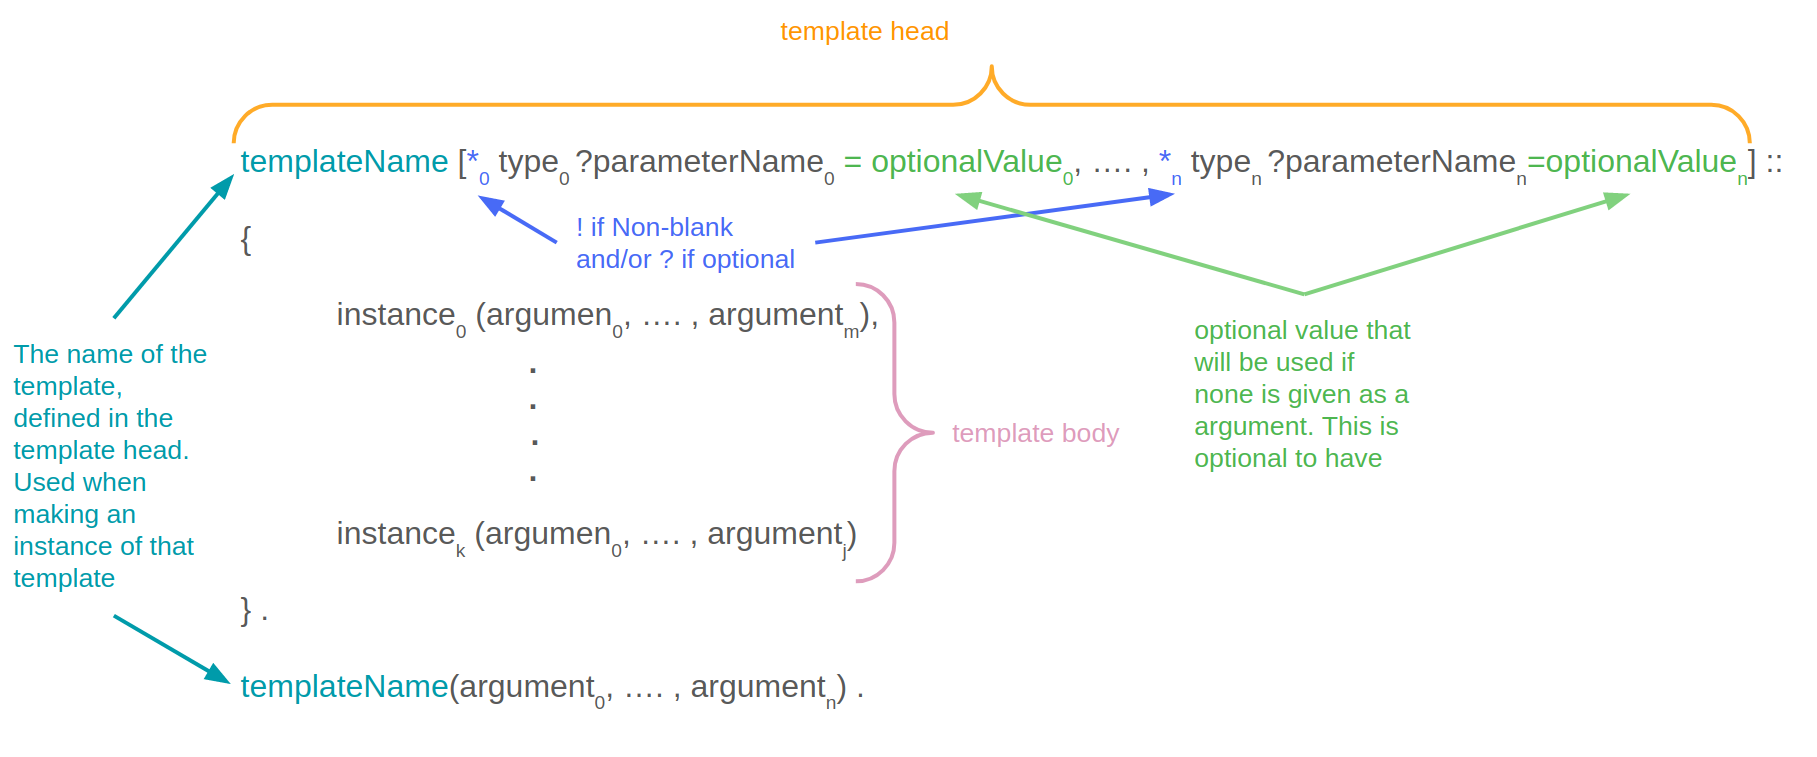
\includegraphics[width=1\textwidth]{stOTTRExample.png}
    \caption{A genralisation showing the syntax of stOTTR}
    \label{fig:stOTTERGenralisation}
\end{figure}

\subsubsection{Types in OTTR}
\label{ottr types} 
Basic types, LUB-types, and list types are the three types that make the OTTR type system. OTTR arranges the types in a subtype relationship, where the set of types are transitive and reflexive. The opposite or inverse of a subtype is a supertype. All the basic types, except for ottr:IRI and ottr:Bot, are common types taken from RDF, RDFS, OWL and XSD standards. ottr:IRI reference to the URI to a resource. ottr:Bot represents the type Bot, a subtype to all other types. In contrast to Bot, OTTR has the type Top, rdfs: Resource, a supertype for all other types.  Top is the default parameter type. If we want the parameter to have another type, we need to add the type before the parameter name explicitly. OTTR throws an error if an argument does not have a compatible type required by the template parameter.  A compatible type to a parameter is either the type that the parameter explicitly states or its subtypes \autocite[5-6]{SLKK_OTTR_2021}.\lhk{Specify the compatibility relation between types, and perhaps give some motivation for the type system in the beginning of this paragraph.}

\para
\emph{LUB} (LUB<>), denoted with ottr:Lub, stands for least upper bound. For every basic type P, there is also a LUB-type LUB<P> such that LUB<P> is a subtype of P. Furthermore, LUB<P> is compatible with all subtypes of P. While P, on the other hand, is compatible with all supertypes of P. Furthermore, OTTR has two different types, \emph{List<>}, denoted with rdf:list, and \emph{NEList<>}, denoted with ottr:NEList. Where NEList stands for non-empty list. The OTTR type system assumes that for each type P, in the set of types, there exists a type List<P> and NEList<P> \autocite[5]{SLKK_OTTR_2021}.

\para
OTTR uses two types of type checking \emph{compatible typing} and \emph{consistent typing}. Compatible typing refers to an argument having a compatible type for the given parameter. Consistent typing, on the other hand, ensures that the parameter is consistently typed. For example, if we have a blank node, which can be any type, and we use that blank node in an instance that excepts an xsd:integer. OTTR will then interpret the blank node as an xsd:integer in the rest of the template, which means sending this blank node as an argument to an instance that expects a xsd:string will result in an error message \autocite[5-6]{SLKK_OTTR_2021}. 

\subsubsection{Terms}
Terms in OTTR are the set of constants and variables where constants include lists, an order collection of terms. In addition to the constant nil, which OTTR uses to denote an empty list. The terms in OTTR are equal to valid RDF terms, such as IRIs, blank nodes, and literals. The only distinction between a variable and a constant term is in the template definition, where the variable occurs in a parameter declaration in the template's signature.\autocite{OTTR_mOTTR}
